\documentclass[12pt,a4paper]{article}
\usepackage[a4paper,total={160mm,250mm}]{geometry}
\usepackage[utf8]{inputenc}
\usepackage{ngerman}
\usepackage{amsmath}
\usepackage{amsthm}
\usepackage{amsfonts}
\usepackage{amssymb}
\usepackage{amscd}
\usepackage{graphicx}
\usepackage{enumerate}
\usepackage{color}
\usepackage{mathtools}
\usepackage[ruled,vlined]{algorithm2e}
\usepackage{subcaption}
\usepackage{listings}
\usepackage{color}
\usepackage{sidecap}

\theoremstyle{definition}
\newtheorem{aufgabe}{Aufgabe}

\theoremstyle{definition}
\newtheorem*{losung*}{Lösung}

\definecolor{mygreen}{rgb}{0,0.6,0}
\definecolor{mygray}{rgb}{0.5,0.5,0.5}
\definecolor{mymauve}{rgb}{0.58,0,0.82}
\definecolor{lightgray}{rgb}{0.9,0.9,0.9}

\lstset{
	backgroundcolor=\color{lightgray},   % choose the background color; you must add \usepackage{color} or \usepackage{xcolor}; should come as last argument
	basicstyle=\footnotesize\ttfamily,        % the size of the fonts that are used for the code
	breakatwhitespace=false,         % sets if automatic breaks should only happen at whitespace
	breaklines=true,                 % sets automatic line breaking
	captionpos=b,                    % sets the caption-position to bottom
	commentstyle=\color{mygreen},    % comment style
	deletekeywords={...},            % if you want to delete keywords from the given language
	escapeinside={\%*}{*)},          % if you want to add LaTeX within your code
	extendedchars=true,              % lets you use non-ASCII characters; for 8-bits encodings only, does not work with UTF-8
	firstnumber=1,                   % start line enumeration with line 1000
	frame=single,	                 % adds a frame around the code
	keepspaces=true,                 % keeps spaces in text, useful for keeping indentation of code (possibly needs columns=flexible)
	keywordstyle=\color{blue},       % keyword style
	language=Python,                 % the language of the code
	morekeywords={*,...},            % if you want to add more keywords to the set
	numbers=left,                    % where to put the line-numbers; possible values are (none, left, right)
	numbersep=5pt,                   % how far the line-numbers are from the code
	numberstyle=\tiny\color{mygray}, % the style that is used for the line-numbers
	rulecolor=\color{black},         % if not set, the frame-color may be changed on line-breaks within not-black text (e.g. comments (green here))
	showspaces=false,                % show spaces everywhere adding particular underscores; it overrides 'showstringspaces'
	showstringspaces=false,          % underline spaces within strings only
	showtabs=false,                  % show tabs within strings adding particular underscores
	stepnumber=1,                    % the step between two line-numbers. If it's 1, each line will be numbered
	stringstyle=\color{mymauve},     % string literal style
	tabsize=4,	                     % sets default tabsize to 2 spaces
	title=\lstname,                   % show the filename of files included with \lstinputlisting; also try caption instead of title
	rangeprefix=\#---,
	rangesuffix=---,
	includerangemarker=false
}

\pagestyle{empty}

\begin{document}
	\section*{Was ist Raytracing?}
	Raytracing bezeichnet eine Methode zur Generierung von realistischen 3D Bildern.
	Dabei kommen unter anderem Reflexions- und Brechungsgesetze aus der Physik zur Anwendung.
	Vor allem aber beruht die Technik auf der Vektorgeometrie wie man sie am Gymnasium unterrichtet.
	Die Idee ist folgende: Wir verteilen einige Objekte (Kugeln, Würfel, etc.) im dreidimensionalen Raum.
	Wir nennen dies die Szene.
	Nun stellt man irgendwo eine Kamera auf.
	Vor der Kamera stellen wir uns eine rechteckige Fläche, die Bildebene, vor.
	Auf die Bildebene zeichnen wir nun die dahinter liegende Szene wie folgt:
	Ausgehend von der Kamera senden wir einen Strahl aus, der die Bildebene durchstösst und dann womöglich auf ein Objekt unserer Szene trifft.
	Trifft der Strahl zum Beispiel auf ein rotes Dreieck, so wird der Durchstosspunkt auf der Bildebene rot eingefärbt.
	Danach senden wir einen weiteren Strahl von der Kamera durch einen anderen Punkt auf der Bildebene und färben den Durchstosspunkt entsprechend ein.
	Wir wiederholen dies bis die ganze Bildebene eingefärbt ist.
	Das so auf der Bildebene generierte Abbild der Szene ist der Output unseres Programms.
	Diese Methode ein Bild zu generieren heisst Raytracing, denn man verfolgt den Strahl.
	\begin{figure}[h!]
		\centering
		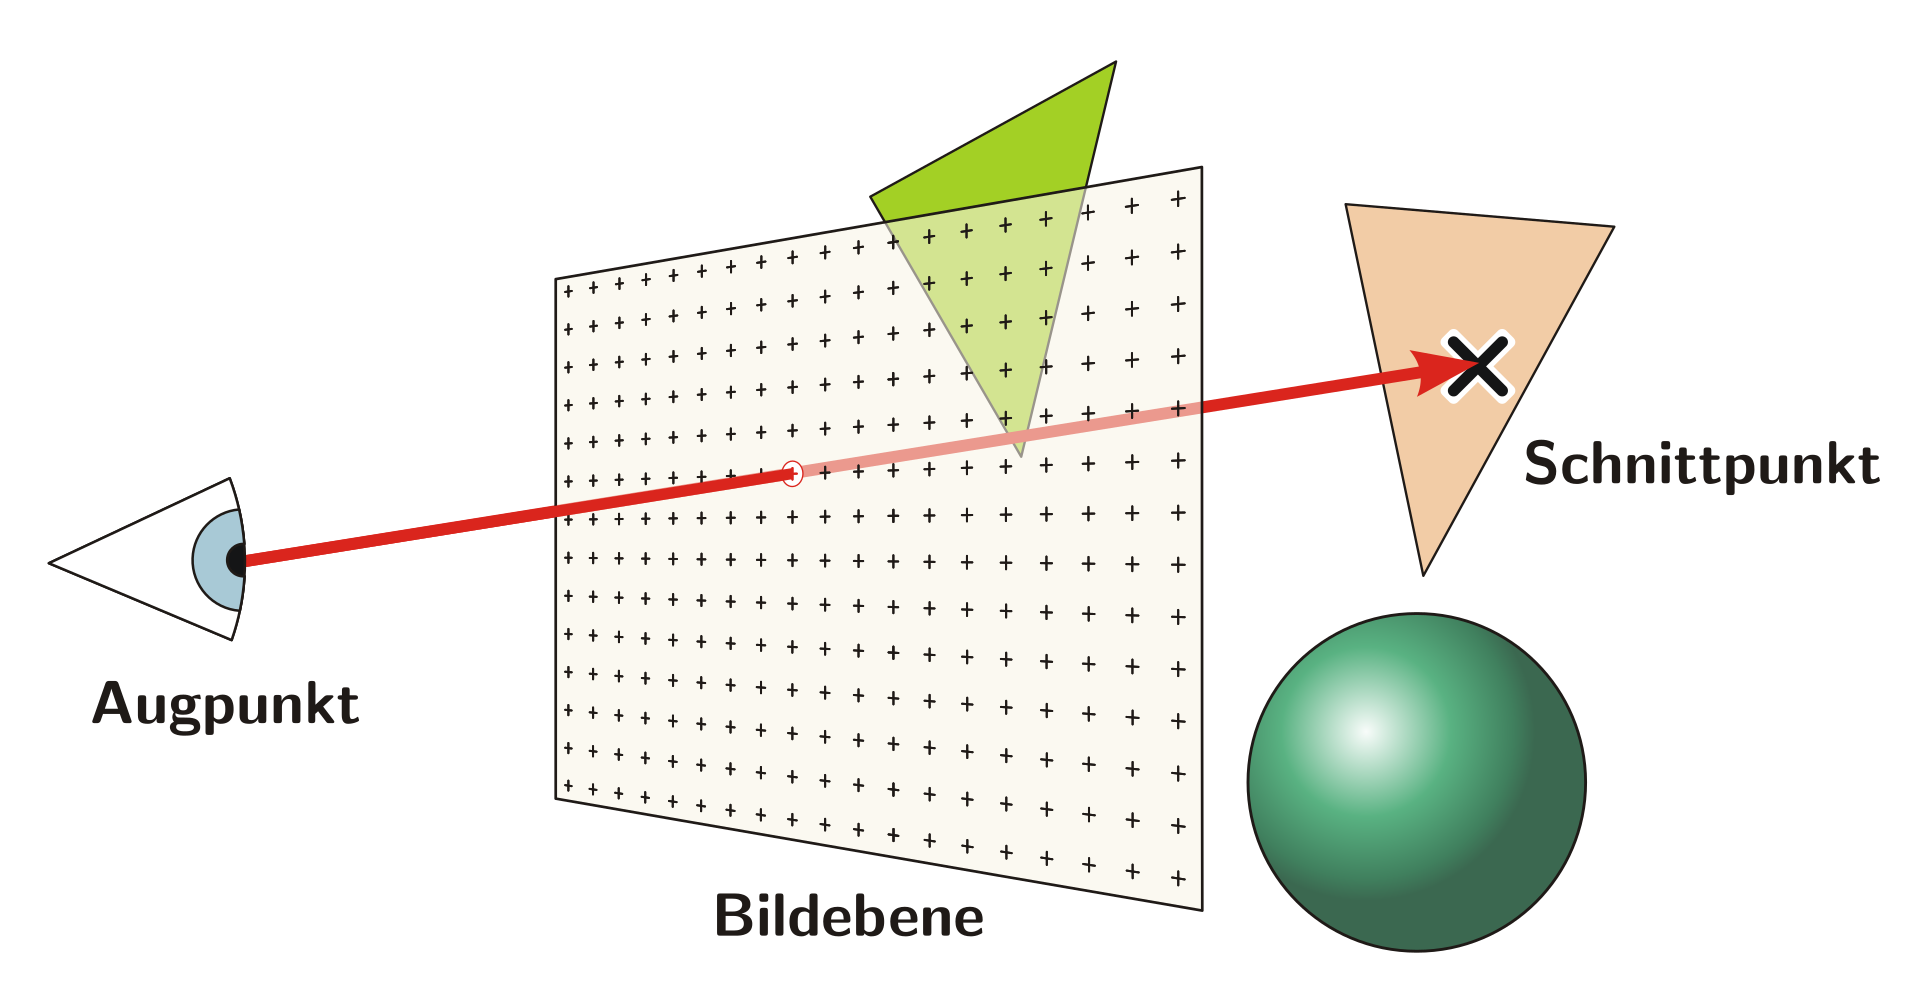
\includegraphics[width=\textwidth]{images/raytracing.png}
		\caption{Raytracing: Es werden Strahlen ausgesendet und deren Schnittpunkte mit Objekten ermittelt. In diesem Fall wir der Durchstosspunkt auf der Bildebene in der Farbe des roten Dreiecks gefärbt.}
		\label{fig:raytracing}
	\end{figure}

	\section*{Worum geht es im Folgenden?}
	Wir wollen nun unser eigenes Raytracing-Programm in Python programmieren.
	Genauer gesagt ist der Raytracing-Algorithmus im Kern schon implementiert.
	Allerdings kennt diese Implementierung noch keine Objekte wie Kugeln, Würfel, Ebenen und so weiter.
	Hier kommen Sie als Leser ins Spiel.
	Sie werden unter Anleitung diese fehlenden Teile ergänzen.
	Es geht darum dem Raytracing-Programm zu sagen, was zum Beispiel eine Kugel ist, wie man deren Schnittpunkt mit einem Strahl berechnet und vieles mehr.
	Am Ende werden wir Bilder wie in Abbildung~\ref{fig:goal} generieren können.
	\begin{figure}[h!]
		\centering
		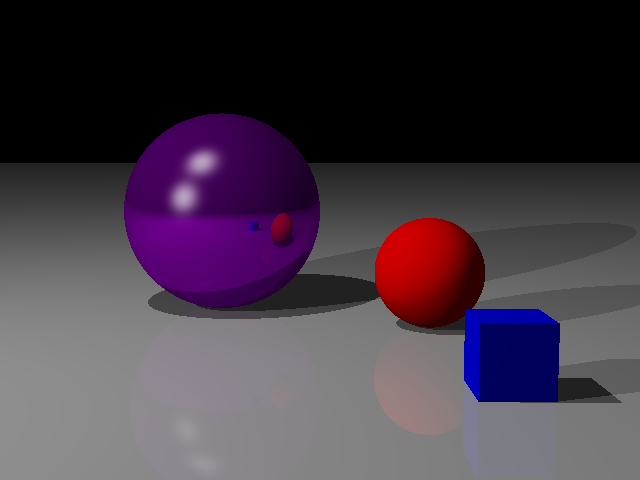
\includegraphics[width=0.75\textwidth]{images/outlook.png}
		\caption{Dieses Bild wurde mit unserem Raytracing-Programm generiert.}
		\label{fig:goal}
	\end{figure}
	Dabei müssen Sie als Leser ausschliesslich die Python-Files im Verzeichnis \texttt{myobject} editieren.
	Die darin enthaltenen Klassen werden dann die verschiedenen Objekt-Typen wie Kugeln, Ebenen und dergleichen beschreiben.
	Ohne hier weiter ins Detail zu gehen, werden wir nun unser erstes Bild generieren.

	\section*{Die Kugel}
	Als Einstieg generieren wir ein Bild bestehend aus folgender Szene:
	Eine Kamera befindet sich an den Koordinaten $(-1,0,1)$ und schaut in Richtung des Punktes $(0,0,1)$, das heisst entlang der x-Achse.
	Zudem platzieren wir eine Kugel mit Mittelpunkt $(1,0,1)$ und Radius $1$.
	Damit schaut die Kamera genau auf die Kugel.
	Diese Szene entspricht dem Python-File \texttt{examples/example1.py}, welches wir nun ausführen. Anstatt eine Kugel sehen wir aber nur ein schwarzes Bild.
	Um die Kugel auch zu sehen, müssen wir zuerst das File \texttt{myobject/sphere.py} bearbeiten.
	Genauer gesagt, muss die Funktion \texttt{intersect(self, ray)} vervollständigt werden.
	Diese soll zu einem gegebenen Strahl dessen nächstgelegenen Schnittpunkt berechnen.
	Man betrachte dazu Abbildung~\ref{fig:sphere_intersect}.
	\begin{figure}[ht]
		\centering
		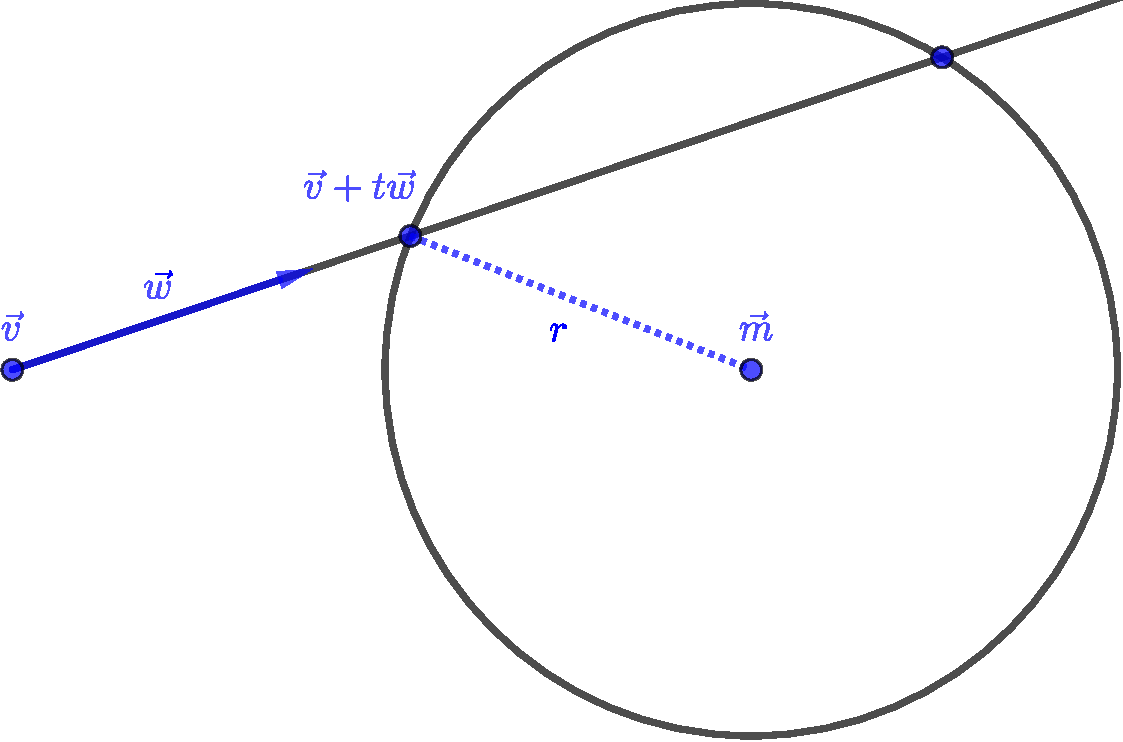
\includegraphics[width=0.5\textwidth]{images/sphere_intersect.pdf}
		\caption{Schnittpunkt von Strahl und Kugel.}
		\label{fig:sphere_intersect}
	\end{figure}
	\begin{aufgabe}\label{aufg:intersect_theory}
		Gegeben Sei ein Strahl mit Ursprung $\vec{v}$ und Richtung $\vec{w}$.
		Überlegen Sie sich die Kugel mit Mittelpunkt $\vec{m}$ und Radius $r$ schneidet.
		Wie erhalten Sie in diesem Fall den Parameter $t>0$, so dass $\vec{v}+t\vec{w}$ gerade dem näherem der beiden Schnittpunkte entspricht?
	\end{aufgabe}
	\begin{losung*}
		Ein beliebiger Punkt auf dem Strahl ist von der Form $\vec{v}+s\vec{w}$ für ein $s>0$.
		So ein Punkt liegt auf der Kugeloberfläche genau dann wenn
		\begin{equation*}
			\lVert\vec{v}+s\vec{w}-\vec{m}\rVert^2=r^2,
		\end{equation*}
		also wenn er den Abstand $r$ zum Mittelpunkt hat.
		Dies ist eine quadratische Gleichung in $s$, das heisst sie ist von der Form
		\begin{equation*}
			as^2+bs+c=0
		\end{equation*}
		für reelle Zahlen $a,b$ und $c$.
		Durch einen Koeffizientenvergleich erhält man
		\begin{equation*}
			a=\rVert\vec{w}\rVert^2,\quad
			b=2\vec{w}\cdot(\vec{v}-\vec{m}),\quad
			c=\lVert\vec{v}-\vec{m}\rVert^2-r^2.
		\end{equation*}
		Falls $b^2-4ac>0$, so existieren genau zwei Schnittpunkte $v+t_1w$ und $v+t_2w$, wobei
		\begin{equation*}
			t_1=\frac{-b-\sqrt{b^2-4ac}}{2a}
			\quad\text{und}\quad
			t_2=\frac{-b+\sqrt{b^2-4ac}}{2a}.
		\end{equation*}
		Wir sind aber nur an positiven Lösungen interessiert, denn wir beschreiben einen Strahl und keine Gerade.
		Sind $t_1$ und $t_2$ beide negativ, so schneidet der Strahl die Kugel nicht.
		Andernfalls ist die kleinste positive Lösung der quadratischen Gleichung unsere Wahl für $t$.
		Der nächstgelegene Schnittpunkt ist entsprechend $v+tw$.
	\end{losung*}
	\begin{aufgabe}\label{aufg:intersect_implementation}
		Öffnen Sie nun das File \texttt{myobject/sphere.py} und implementieren Sie die Funktion \texttt{intersect(self, ray)} gemäss Ihren Überlegungen aus Aufgabe~\ref{aufg:intersect_theory}.
		Lassen Sie anschliessend das Skript \texttt{examples/example1.py} nochmals laufen.
		Nun sollten Sie die Kugel sehen.
	\end{aufgabe}
	\begin{losung*}
		Die Lösung könnte zum Beipiel so aussehen:
		\lstinputlisting[linerange=intersect\-begin-intersect\-end]{../object/sphere.py}
		Zusätzlich zu unserer Lösung von Aufgabe~\ref{aufg:intersect_theory} haben wir hier noch überprüft, ob der Strahl am Schnittpunkt in die Kugel eintritt (und nicht etwa austritt).
		Nur diese Lösung lassen wir zu.
		Wir werden später sehen, warum das nützlich ist.
		Das so generierte Bild ist in Abbildung~\ref{fig:solution_sphere} gezeigt.
		\begin{figure}[ht]
			\centering
			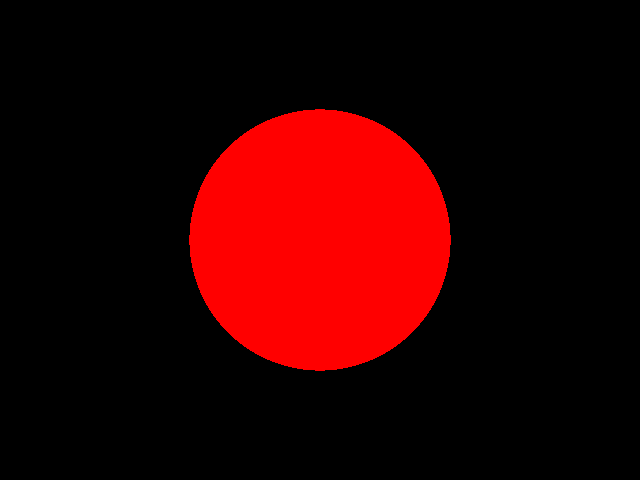
\includegraphics[width=0.5\textwidth]{images/example1.png}
			\caption{Lösung der Aufgabe~\ref{aufg:intersect_implementation}.}
			\label{fig:solution_sphere}
		\end{figure}
	\end{losung*}
	Unsere Kugel sieht momentan eher wie eine Kreisscheibe aus, weil wir der Kugel an jedem Punkt den selben Farbwert geben.
	Das wollen wir nun ändern indem wir eine diffuse Lichtreflexion simulieren.
	Das Python-File \texttt{examples/example2.py} platziert zu diesem Zweck eine Punktförmige Lichtquelle an den Koordinaten $(0,0,10)$.
	Diese wollen wir nun in die Berechnung der Farbwerte miteinbeziehen:
	Die Punkte auf der Kugeloberfläche, welche der Lichtquelle zugewandt sind, sollen heller sein.
	Die wichtigsten Begriffe sind das \textit{Skalarprodukt} und der \textit{Normalenvektor} auf die Kugeloberfläche.
	Man betrachte dazu Abbildung~\ref{fig:sphere_diffuse}.
	\begin{SCfigure}[2][!h]
		\centering
		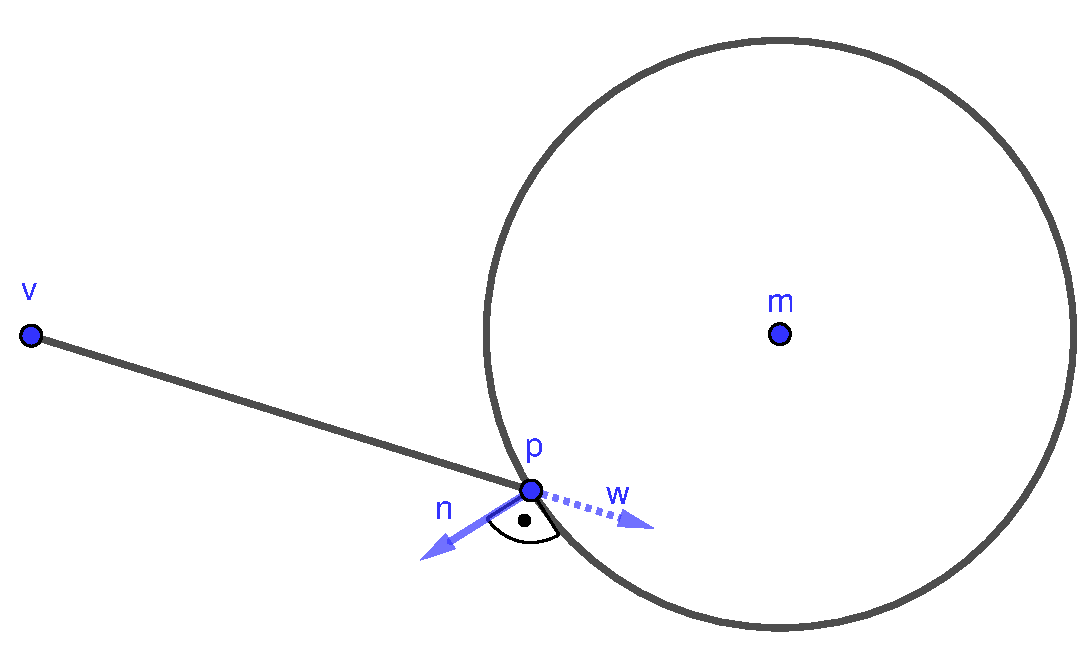
\includegraphics[width=0.3\textwidth]{images/sphere_diffuse.pdf}
		\caption{Die Lichtquelle befindet sich am Punkt $\vec{v}$. Wir wollen den Farbwert am Punkt $\vec{p}$ auf der Kugel berechnen. Der Vektor $\vec{n}$ an diesem Punkt soll rechtwinklig zur Kugeloberfläche sein, nach aussen Zeigen und Länge $1$ haben. Wir nennen $\vec{n}$ den Normalenvektor an $\vec{p}$.}
	\label{fig:sphere_diffuse}
	\end{SCfigure}
	Zu einer gegebenen Lichtquelle am Punkt $\vec{v}$ und einem Beliebigen Punkt $\vec{p}$ auf der Kugel berechnen wir eine Zahl $c\in\left[0,1\right]$ welche die Helligkeit an diesem Punkt beschreibt.
	Dabei heisst $c=1$ maximale Helligkeit und $c=0$ heisst minimale Helligkeit, also Schwarz.
	Das geht folgendermassen:
	\begin{equation}\label{eq:diffuse_coefficient}
		c=\max\left(-\vec{n}\cdot\vec{w}, 0\right),\quad
		\vec{w}=\frac{\vec{p}-\vec{v}}{\lVert\vec{p}-\vec{v}\rVert}.
	\end{equation}
	\begin{aufgabe}\label{aufg:diffuse_coefficient}
		Ist die Berechnung von $c$ in Gleichung~\eqref{eq:diffuse_coefficient} sinnvoll? Erklären Sie.
	\end{aufgabe}
	\begin{losung*}
		Da sowohl $\vec{n}$ als auch $\vec{w}$ Länge $1$ haben, gilt wie verlangt $c\in\left[0,1\right]$.
		Der Vektor $\vec{w}$ beschreibt gerade die Einfallsrichtung des Lichtes am Punkt $\vec{p}$.
		Ist diese rechtwinklig auf die Kugeloberfläche, so haben wir $c=1$, also maximale Helligkeit.
		Je kleiner der Einfallwinkel des Lichtes, desto kleiner wird $c$, bis schliesslich alle  Punkte auf der der Lichtquelle abgewandten Seite die Helligkeit $c=0$ haben.
	\end{losung*}
	\begin{aufgabe}\label{aufg:diffuse_implementation}
		Öffnen Sie nun das File \texttt{myobject/sphere.py} und implementieren Sie die Funktion \texttt{get\_normal(self, p)}, nach aussen zeigenden Normalenvektor $\vec{n}$ der Lange $1$ am Punkt $\vec{p}$ zurück gibt.
		Lassen Sie anschliessend das Skript \texttt{examples/example2.py} laufen.
	\end{aufgabe}
	\begin{losung*}
		Die Lösung könnte zum Beipiel so aussehen:
		\lstinputlisting[linerange=get\_normal\-begin-get\_normal\-end]{../object/sphere.py}
		Das generierte Bild in Abbildung~\ref{fig:solution_diffuse} sieht schon viel interessanter aus.
		Die Lichtquelle befindet sich über der Kugel und beleuchtet nur deren obere Hälfte.
		\begin{figure}[ht]
			\centering
			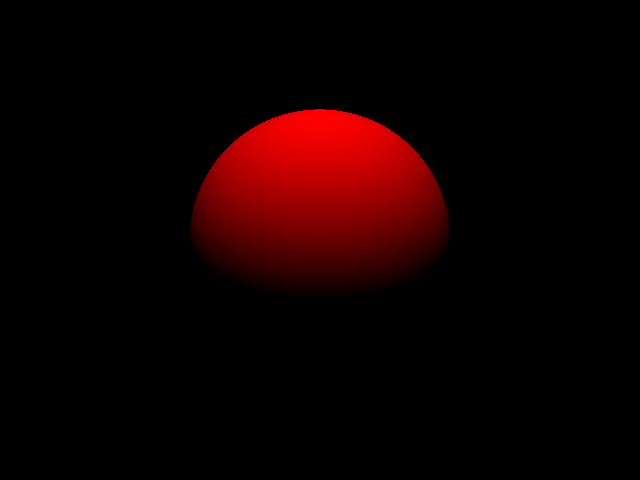
\includegraphics[width=0.5\textwidth]{images/example2.png}
			\caption{Lösung der Aufgabe~\ref{aufg:diffuse_implementation}.}
			\label{fig:solution_diffuse}
		\end{figure}
	\end{losung*}
\end{document}
